\section{Mekanisk montering} \label{sec:mekanisk_montering}

Der er gjort en dyd i at montere enhederne og styreenhederne stabilt og solidt så de ikke rasler af når bilen kører. Ligeledes er der anvendt et etagesystem bestående af bl.a. plexiglas og nylonfødder, så der ikke kan opstå kortslutninger. Ved montering af bilens afstandssensorer er det valgt at placere dem så tæt ved hinanden som muligt for at undgå en blind vinkel lige foran og lige bagved bilen. På figur \ref{fig:billede_af_bil} ses bilen som og en forklaring af hvad de enkelte enheder er. Det skal lige noteres at biles batteri ikke er monteret på bilen på dette billede.\\
Ved projektforløbets afslutning var det desværre ikke lykkedes at få tilkoblet servomotoren til forhjulene, så den er blot placeret ved forhjulene, så det stadig er muligt at se at den reagerer på brugerinput.

\begin{figure}[h]
\centering
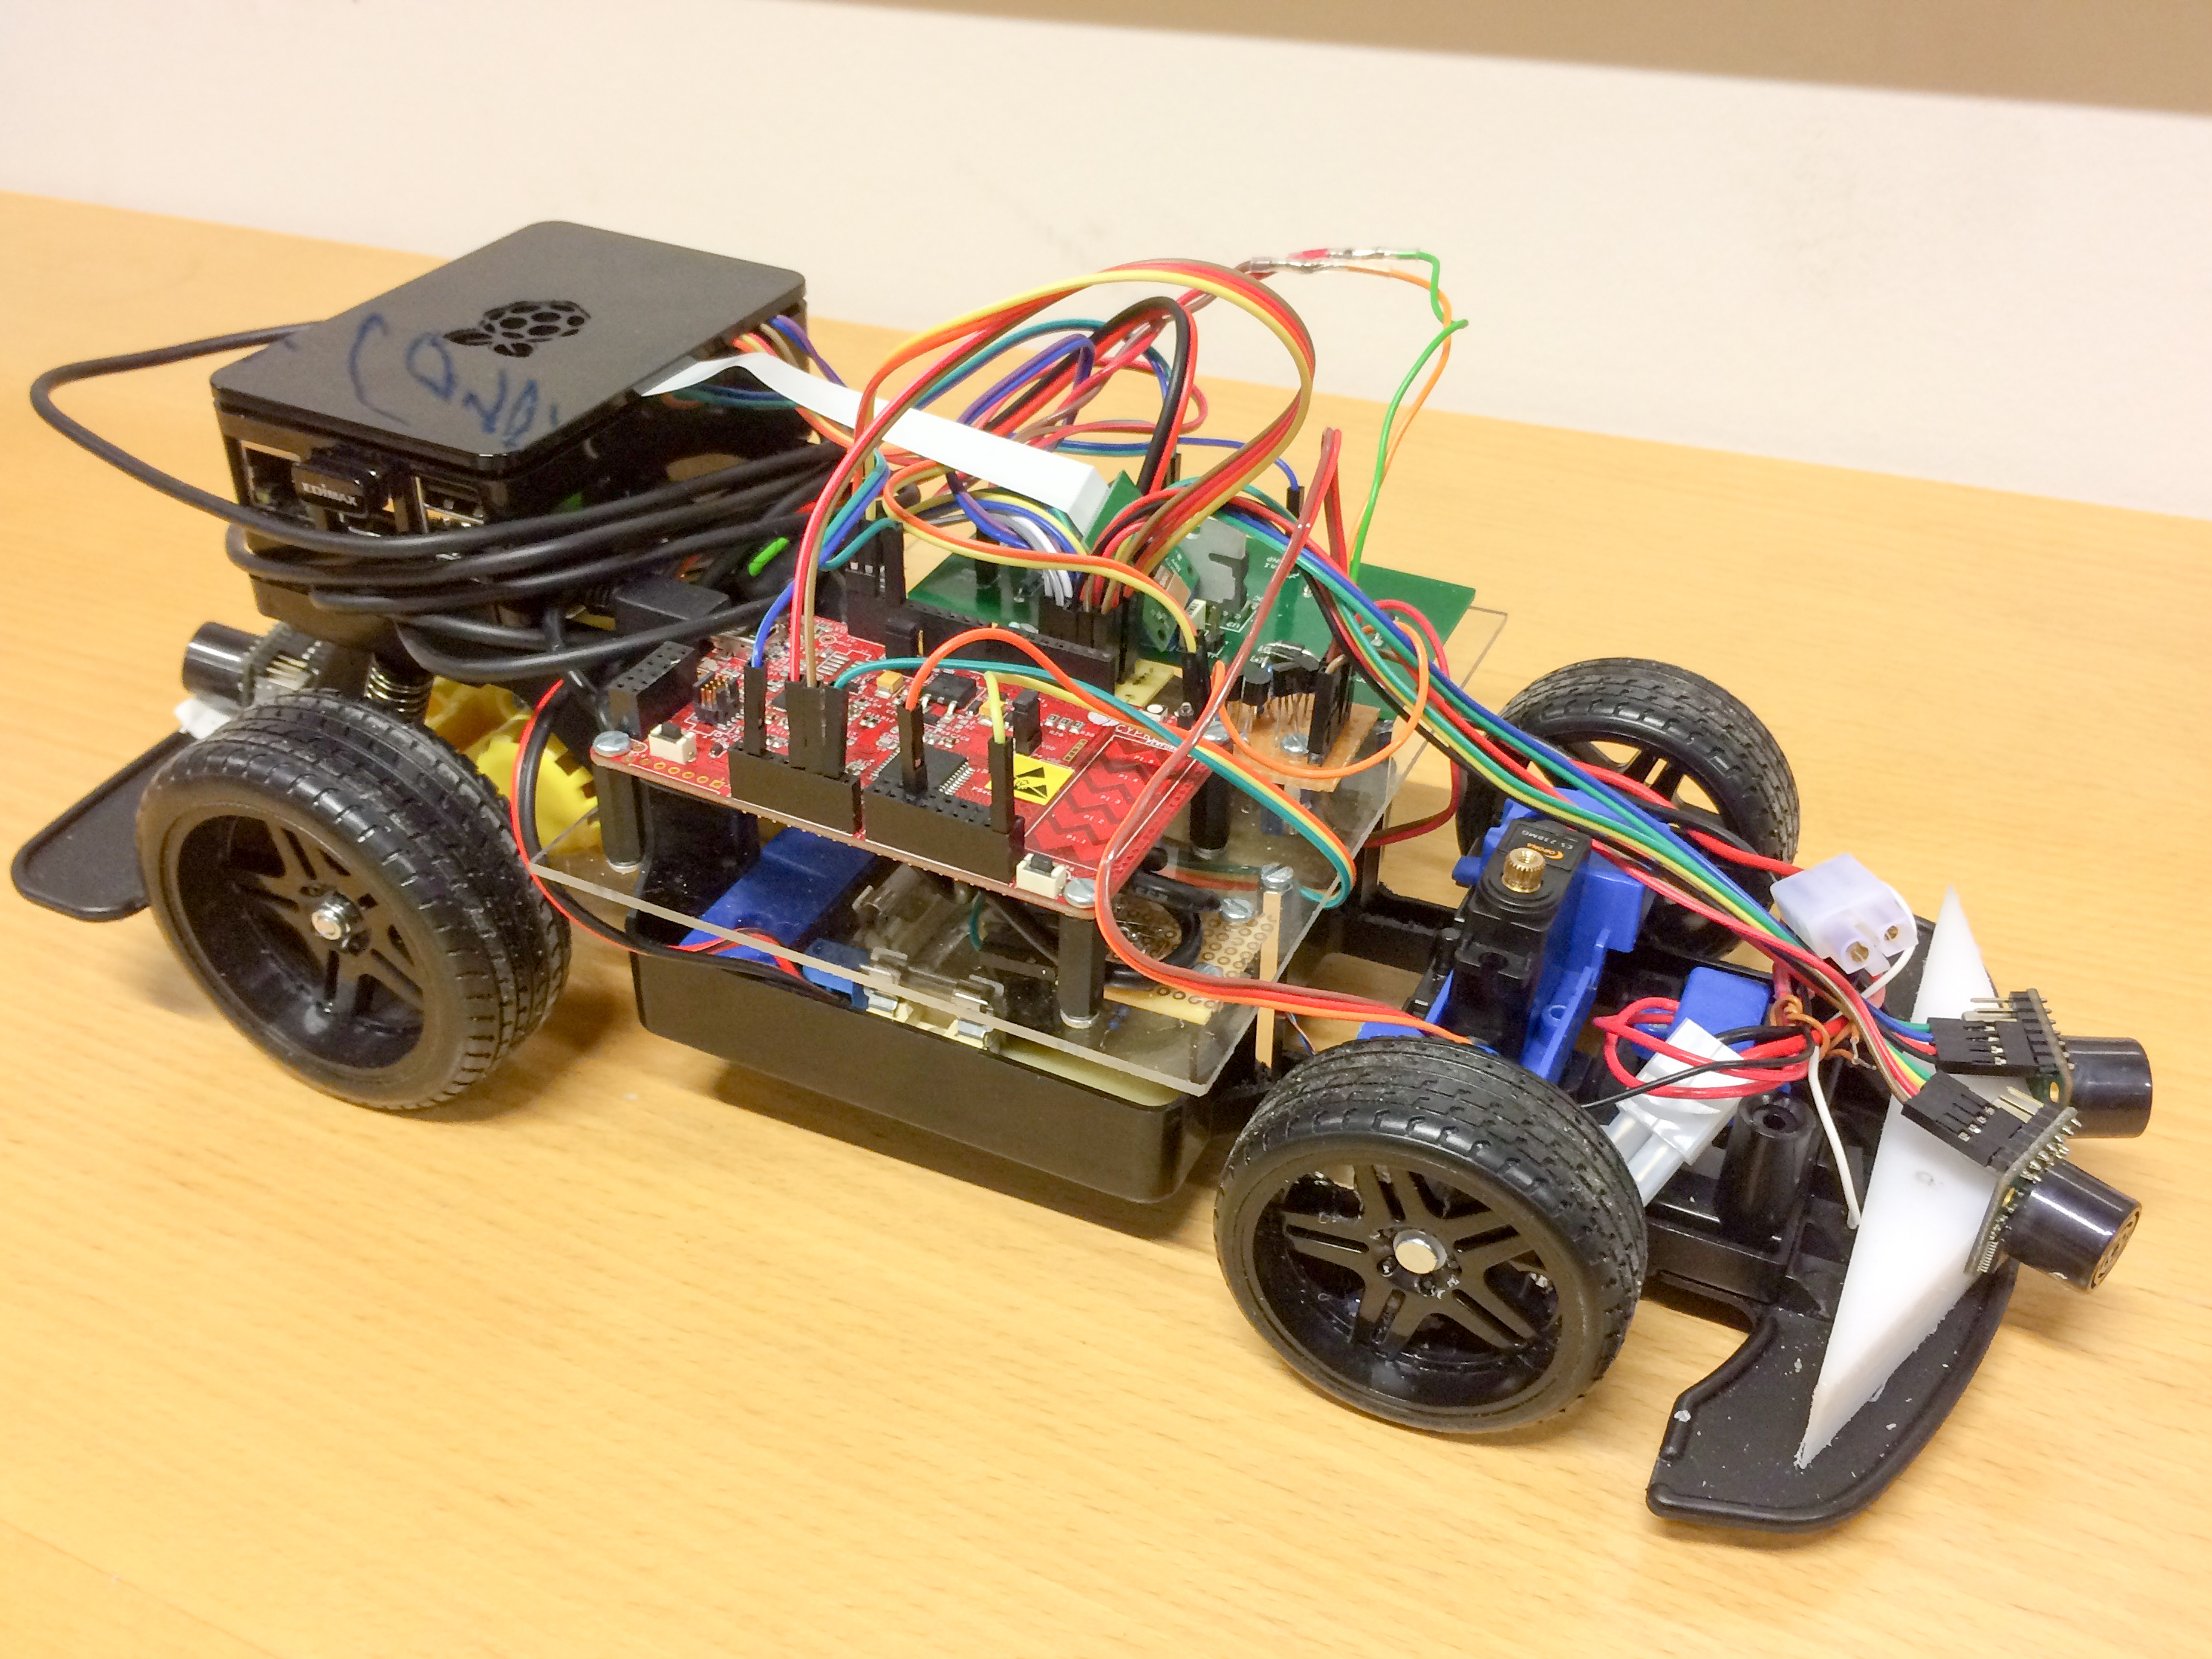
\includegraphics[width=\textwidth -1cm]{../fig/billeder/billede_af_bil.jpg}
\caption{Bilen med montering af komponenter.}
\label{fig:billede_af_bil}
\end{figure}

\begin{table}[h]
\begin{tabularx}{\textwidth}{Z Z}
\begin{packed_enum}
\item PSU
\item Forreste afstandssensorer
\item PSoC
\item H-Bro
\item Buffer til servomotor
\item Tachometer
\end{packed_enum}
&
\begin{packed_enum}
\setcounter{enumi}{6}
\item I2C-bus
\item Pi
\item Bageste afstandssensorer
\item Servomotor
\item Wi-Fi dongle
\end{packed_enum}
\end{tabularx}
\end{table}
